%\documentclass[12pt,a4paper]{report}
\documentclass[12pt,a4paper]{article}

\usepackage[brazil]{babel}
\usepackage[utf8]{inputenc}
\usepackage[T1]{fontenc}
\usepackage{graphicx,url}
\usepackage{hyperref}
%\usepackage{mathptmx}
\usepackage{lipsum}
\usepackage{booktabs}
\usepackage{pifont}
\usepackage{textcomp}
\usepackage{amsmath,amssymb}
\usepackage{listings}
\usepackage[scaled=0.8]{beramono}
\usepackage{xspace}
\usepackage{pdfpages}

\pdfgentounicode=1

\newcommand{\HRule}{\rule{\linewidth}{0.5mm}}

\begin{document}

\begin{titlepage}

\begin{center}


\includegraphics[width=1.0\textwidth]{img/unb_logo.jpg}~\\[1cm]

\textsc{\Large Programação Paralela}\\[0.5cm]

% Title
\HRule\\[0.4cm]
{\huge \bfseries Relatório do Exercício 3\\[0.4cm]}
\HRule\\[1.5cm]

% Author and Supervisor
\begin{minipage}{0.4\textwidth}
\begin{flushleft} \large
\textit{Autor:}\\
\small{Alexandre Lucchesi Alencar}
\end{flushleft}
\end{minipage}
\begin{minipage}{0.4\textwidth}
\begin{flushright} \large
\textit{Professor:}\\
\small{George Luiz Medeiros Teodoro}
\end{flushright}
\end{minipage}

\vfill

% Bottom of the page
{\large \today}

\end{center}

\end{titlepage}



\section{Introdução}
Este relatório tem como objetivo apresentar os resultados obtidos a partir da
execução do segundo exercício de programação paralela~\cite{exercise}, que
consiste na paralelização do algoritmo \emph{Pi de Monte Carlo} utilizando a
biblioteca \texttt{pthreads}. Primeiramente, os aspectos principais do
algoritmo desenvolvido e a estratégia de paralelização utilizada é apresentada.
Em seguida, é realizada uma análise de desempenho comparando os tempos de
execução do algoritmo em diversas configurações, isto é, variando-se o número
de lançamentos (pontos) e o número de \textit{threads}.  O código-fonte
completo deste trabalho (incluindo os arquivos \LaTeX\xspace que compõem este
relatório) estão publicamente disponíveis no
GitHub~\footnote{\url{https://github.com/alexandrelucchesi/parallel-programming-ex02}}.

\subsection{\textit{Hardware} Utilizado}
\label{sec:hardware}

\begin{itemize}
    \item Processador: Intel Core i7
    \item Velocidade: 2 GHz
    \item Número de processadores: 1
    \item Número de \textit{cores} reais: 2
    \item Número de \textit{cores} virtuais: 4 (HyperThreading)
    \item L1 cache: 32KB
    \item L2 cache (per core): 256KB
    \item L3 cache: 4MB
\end{itemize}


\section{O Algoritmo}
Além do programa principal, foi desenvolvido um \textit{script bash} para
automatizar os testes da aplicação. Esses artefatos são descritos a seguir.

\begin{itemize}
	\item \texttt{main.c}: programa em C contendo o código-fonte da aplicação. Após compilado com as respectivas diretivas
		(\texttt{-lpthread -lmath} --- vide Makefile) recebe via
		\texttt{scanf()} dois argumentos: o número de \textit{threads} a serem
		criadas e a quantidade de lançamentos a serem realizados. A saída do
		programa tem duas linhas: a primeira contém o valor aproximado de Pi e
		a segunda, o tempo de execução do algoritmo em microsegundos.
	\item \texttt{test.sh}: \textit{script} desenvolvido para automatizar os
		testes da aplicação. Recebe como entrada 4 argumentos, em ordem:
		\begin{itemize}
			\item \texttt{max\_threads}: número máximo de \textit{threads}. O
				\textit{script} varia o número de \textit{threads} de 1 até
				\texttt{max\_threads}.
			\item \texttt{max\_tosses}: ordem máxima do número de lançamentos, isto
				é, o \textit{script} executa a aplicação variando o 
				número de lançamentos, começando em $10^2, 10^3$ até $10^{max\_tosses}$.
			\item \texttt{max\_runs}: número máximo de vezes em que o programa
				deve ser executado em uma mesma configuração.
			\item \texttt{max\_time}: \textit{timeout} de execução, ou seja, se o
				programa não encerrar a execução nesse tempo, ele é finalizado.
		\end{itemize}
\end{itemize}

\subsection{Geração de números aleatórios}
Como o método de aproximação do valor de pi é baseado no Método de Monte Carlo,
é necessária a geração de números aleatórios de ponto-flutuante. Além disso, a
função que gera esses números tem que ser \textit{thread safe}, uma vez que o
algoritmo será paralelizado e o código chamado por várias \textit{threads} ao
mesmo tempo. Por isso, utilizou-se a função \texttt{rand\_r(unsigned int *)}.

A função inicializadora, \texttt{srand(unsigned int seed)}, foi executada uma
vez por \textit{thread}. Inicialmente, utilizou-se como semente para
\texttt{srand} o resultado de uma função temporal (\texttt{time(NULL)}), porém,
os resultados de pi em múltiplas execuções do programa quando executado a
partir do \textit{script} estava igual. Acredita-se que isso se deve ao fato
das várias execuções serem realizadas em um intervalo de tempo muito pequeno,
pois, acrescentando-se um \texttt{sleep(1)} entre as chamadas, os resultados
começaram a variar.

Apesar de correta, a solução com \texttt{sleep()} não é ideal, pois deixa a
execução dos testes muito lenta, sobretudo se o conjunto de testes for
abrangente (vide Seção~\ref{sec:resultados}). Dessa forma, somou-se ao resultado
de \texttt{time(NULL)} um fator para introduzir aleatoridade que é único entre
várias execuções do programa: o valor de \texttt{getpid()}.

\subsection{Política de escalonamento}
Procurou-se similar a política de escalonamento estática encontrada na
biblioteca OpenMP.  Dessa forma, tenta-se dividir igualmente o trabalho entre
as \textit{threads} antes da criação ou execução das mesmas. Por exemplo, se a
entrada do programa for 2 \textit{threads} e 1000 lançamentos, atribui-se
previamente a cada \textit{thread} o cálculo de 500 lançamentos. Caso a divisão
não seja exata, ou seja, se a entrada do programa for 2 \textit{threads} e 1005
lançamentos, o excedente (resto da divisão) é atribuído à primeira
\textit{thread} criada.


\subsection{Parâmetros de entrada}
Se o número de \textit{threads} especificado for menor ou igual a 1, nenhuma
\textit{thread} é criada e o programa é executado de forma sequencial. É válido
ressaltar que isso não implicou em redundância de código-fonte, ou seja, no
\emph{modo sequencial} é executada a mesma função cujo ponteiro seria passado
para \texttt{pthread\_create()}, porém, sem o \textit{overhead} de criação e
finalização de \textit{threads}.


\subsection{Tipos das variáveis}
Com o objetivo de se preservar ao máximo os dados provenientes das computações
e mitigar a perda de precisão por truncamento ou resultados errôneos por
\textit{overflow}, usou-se em toda a aplicação os tipos \texttt{unsigned long
long int} e \texttt{long long int} para valores inteiros, e \texttt{long
double} para valores de ponto flutuante. Utilizou-se \texttt{typedef}s para tornar o código menos verboso e mais 
legível:

\begin{verbatim}
typedef unsigned long long int ulli;
\end{verbatim}


\section{Resultados}
\label{sec:resultados}
Executou-se o \textit{script} de testes (\texttt{test.sh}) passando-se como
argumentos: 6 \textit{threads}, $10^{12}$ lançamentos, 5 execuções por
configuração e \textit{timeout} de 24 minutos. Além disso, utilizou-se o
utilitário de linha de comando \texttt{time} para calcular o tempo total de
execução dos testes. O resultado é apresentado a seguir.

\begin{verbatim}
$ time sh test.sh 6 12 5 1440

real    633m8.800s
user    1503m45.812s
sys     1m9.481s
\end{verbatim}

O valor \texttt{real} é o tempo real (``relógio de parede'') transcorrido desde
o início da execução do programa até seu término (incluindo períodos de
bloqueio, etc). Por outro lado, os valores de \texttt{user} e \texttt{sys} se
referem ao tempo de CPU usado pelo processo em modo usuário e modo
\textit{kernel}, respectivamente. Dessa forma, a execução dos testes
responsáveis por gerar as tabelas de \textit{benchmark} levou quase 11 horas
para ser concluída.

O \textit{script} \texttt{test.sh} gera como saída $2 \times max\_threads$
arquivos no formato CSV\@ (no exemplo acima, 12 arquivos). Cada tabela é
indexada pelo número de lançamentos (no exemplo acima, de $10^2$ à $10^{12}$) e
o número da execução (no exemplo acima, de 1 a 5).  Metade possui o prefixo
\texttt{pi\_{n}}, onde \texttt{n} é o número de \textit{threads} utilizado,
representando os valores aproximados de pi calculados. A outra metade possui
prefixo \texttt{time\_{n}}, e contém os valores dos tempos de execução. O valor
\texttt{*} representa um \textit{timeout}. Em poucas palavras, tem-se 2 arquivos
por quantidade de \textit{threads} contendo as duas saídas do programa: o valor
estimado de pi e o tempo de execução do algoritmo.

As tabelas a seguir apresentam os resultados dos testes. Observa-se que para uma
quantidade de lançamentos pequena ($10^2$ e $10^3$), o tempo de execução do
algoritmo sequencial é melhor do que nas demais configurações. Isto ocorre
porque os ganhos obtidos da paralelização do algoritmo não são suficientes para
cobrir o custo de se criar as \textit{threads}. Ao aumentar o número
de lançamentos para $10^4$, observa-se que o desempenho do algoritmo sequencial
já perde para algumas configurações, sendo inferior ao obtido com 3 e 4
\textit{threads}. A partir de $10^5$ lançamentos, o desempenho do algoritmo
sequencial se torna inferior a todas as demais configurações.

É importante notar que para o algoritmo sequencial e para as configurações 2 e 3
\textit{threads}, o programa excedeu o tempo máximo de execução pré-estabelecido
(24 minutos). No entanto, para as configurações 4, 5 e 6 \textit{threads}, esse
tempo não foi atingido, evidenciando que o algoritmo paralelizado é escalável.
Além disso, observando-se os tempos de execução quando o número de lançamentos é
alto ($10^{10}$ e $10^{11}$), conclui-se que o maior desempenho é alcançado
utilizando-se 4 \textit{threads}. Isso está relacionado com o fato de que o
processador utilizado possui 2 \textit{cores} em
HyperThreading~\ref{sec:hardware}.

Em linhas gerais, para $10^{6}$ lançamentos e 4 \textit{threads}, foi possível
obter o \textit{speedup} máximo: $\approx 252\%$. Em contrapartida, para
$10^{2}$ lançamentos e 6 \textit{threads}, ocorreu o pior \textit{speedup}:
$\approx 4.5\%$. Esse resultado era esperado, uma vez que o custo de se
gerenciar 6 \textit{threads} para calcular apenas 100 números é muito alto.

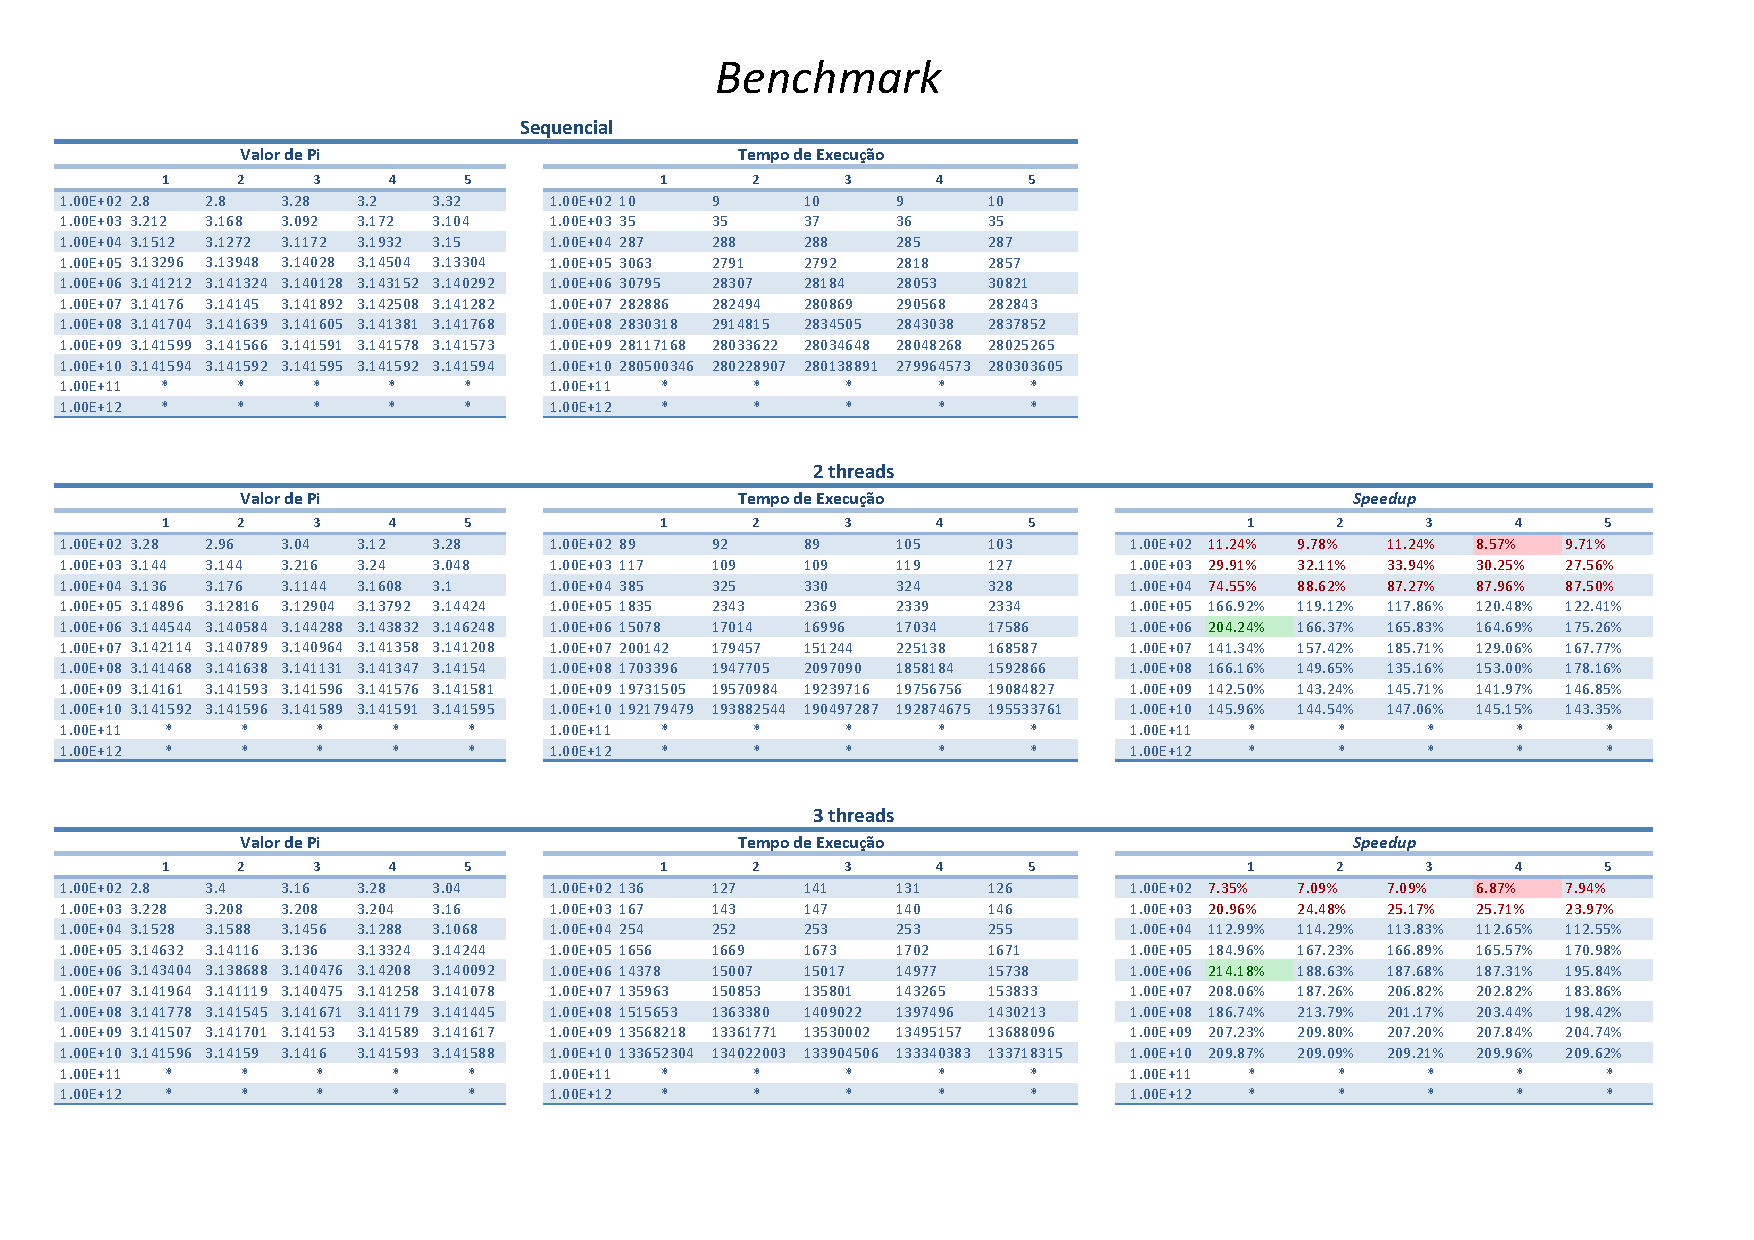
\includepdf[pages={1-},scale=1.0,landscape=true]{bench.pdf}

%A Tabela~\ref{table:bench-sched-chunk} apresenta os resultados da primeira
%análise. Nota-se que em todos os casos, o tamanho de \textit{chunk} ótimo foi
%1.  Isso contrariou as expectativas, pois esperava-se obter como tamanho ótimo
%para o \textit{chunk} um valor que se aproximasse do tamanho da \textit{cache},
%para se beneficiar do \emph{alinhamento de cache}~\cite{class-notes}. Além
%disso, observa-se que o escalonamento estático apresenta desempenho médio
%superior ao dinâmico e ao guiado, e que o impacto de desempenho provocado pela
%leitura dos dados é irrisório, sendo em média inferior à 0.1s.
%
%%\begin{table}[h!]
%%\footnotesize
%%\centering
%%\caption{Tamanho de \textit{chunk} variável e número de \textit{threads} fixo (em 4).}
%%\label{table:bench-sched-chunk}
%%\input{./bench_sched_chunk.tex}
%%\end{table}
%
%A Tabela~\ref{table:bench-sched-thread} apresenta os resultados da segunda
%análise. Observa-se dois valores aparentemente absurdos de tempo de resposta com
%escalonamento dinâmico e uma \textit{thread}: 680.678471s e 680.679593s. No
%entanto, esses valores apareceram nos resultados porque o \textit{laptop}
%``dormiu'' devido à inatividade enquanto executava o algoritmo.
%
%%\begin{table}[h!]
%%\footnotesize
%%\centering
%%\caption{Tamanho de \textit{chunk} fixo (em 256) e número de \textit{threads}
%%variável.}
%%\label{table:bench-sched-thread}
%%\input{./bench_sched_thread.tex}
%%\end{table}
%
%O \textit{speedup} de um programa paralelo é definido como~\cite{main-book}:
%
%$$S = \frac{T_{serial}}{T_{parallel}}$$
%
%Por motivos de simplificação, a Tabela~\ref{table:speedup} apresenta a relação
%entre o \textit{speedup} obtido e o número de \textit{threads} executadas apenas
%para o escalonamento estático, uma vez que as outras políticas apresentaram
%ganhos similares. Observa-se que ao se utilizar duas \textit{threads} foi
%possível obter um ganho significativo de desempenho ($\approx 72\%$). A partir
%de três \textit{threads} o ganho sofreu atenuação e manteve uma certa
%uniformidade. Acredita-se que esse comportamento ocorreu devido as
%características do processador utilizado (vide Seção~\ref{sec:hardware}), que só
%possui 2
%\textit{cores}.
%
%\begin{table}[h!]
%\footnotesize
%\centering
%\caption{\textit{Speedup} x \textit{threads}.}
%\label{table:speedup}
%\begin{tabular}{@{}cccccccc@{}}
%\toprule
%\textit{Threads} & 2 & 3 & 4 & 5 & 6 & 7 & 8 \\ \midrule
%\textit{Speedup} & 0.717707 & 0.548823 & 0.564227 & 0.573196 & 0.580434 & 0.567042 & 0.581778 \\ \bottomrule 
%\end{tabular}
%\end{table}


\section{Conclusão}
Este trabalho possibilitou uma maior compreensão acerca da biblioteca
\texttt{pthreads} e sobre algumas das dificuldades encontradas no contexto de
programação paralela. O algoritmo \textit{Pi de Monte Carlo} foi otimizado a
partir da aplicação de técnicas de programação para um maior aproveitamento dos
recursos computacionais que levaram a ganhos de desempenho. Uma análise dos
tempos de execução do algoritmo evidenciou ganhos de desempenho
(\textit{speedup}) de até 252\% em relação à versão sequencial.

Por fim, é válido ressaltar que o o \textit{design} da aplicação (incluindo o
\textit{script} \texttt{test.sh}) permite variar de forma fácil as condições de
teste, permitindo a reprodução dos experimentos apresentados neste trabalho e
facilitando a experimentação com novas configurações. 

\bibliographystyle{plain}
\bibliography{references.bib}

\end{document}








